\section{Análise Univariada}

\texto

\begin{figure}[h!]
\centering
{\scriptsize Tabela 1: Número de municípios amostrados, registros e espécies nos bancos de dados: WAV = Wikiaves, SLI = SpeciesLink, WAV2 = WAV com municípios redundantes em SLI.}
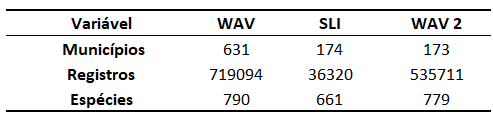
\includegraphics{Tabelas/1.png}
\end{figure}

\texto

\texto

\newpage

\subsection{Registros por Município}

\begin{figure}[h!]
\centering
{\scriptsize Tabela 2: Estatísticas de tendência central e dispersão para o número de registros por município em cada banco de dados: WAV = Wikiaves, SLI = SpeciesLink, WAV2 = WAV com municípios redundantes em SLI. Valores de média (m) e desvio-padrão (dp) em Log10 foram retrotransformados (Retro). min-max = valores extremos, q1-q3 = quartis.}
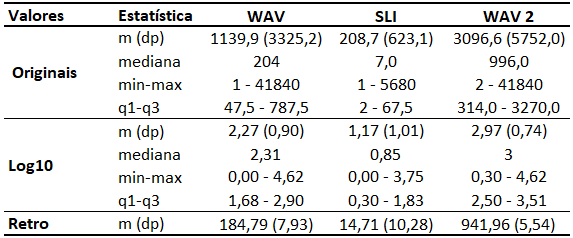
\includegraphics{Tabelas/2.png}
\end{figure}

\texto

\begin{figure}[h!]
\centering
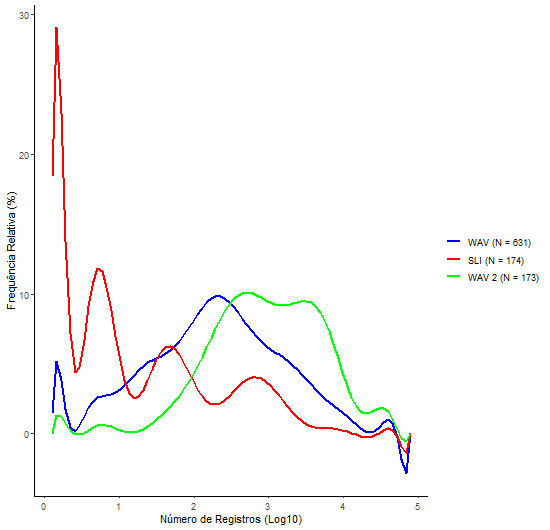
\includegraphics[height = 8cm]{Imagens/113.png}
\\{\scriptsize Figura 1: Distribuição de municípios em classes segundo o número de registros (Log10), em cada banco de dados: WAV = Wikiaves, SLI = SpeciesLink, WAV2 = WAV com municípios redundantes em SLI. n = número de municípios.  }
\end{figure}

\subsection{Espécies por Município}

\begin{figure}[h!]
\centering
{\scriptsize Tabela 3: Estatísticas de tendência central e dispersão para o número de espécies por município em cada banco de dados: WAV = Wikiaves, SLI = SpeciesLink, WAV2 = WAV com municípios redundantes em SLI. Valores de média (m) e desvio-padrão (dp) em Log10 foram retrotransformados (Retro). min-max = valores extremos, q1-q3 = quartis.}
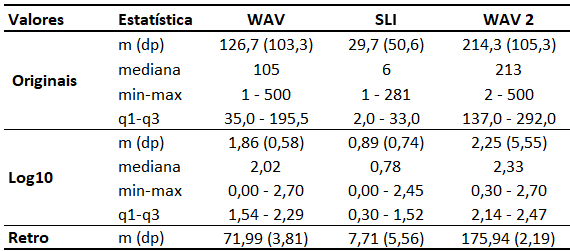
\includegraphics{Tabelas/3.png}
\end{figure}

\texto

\begin{figure}[h!]
\centering
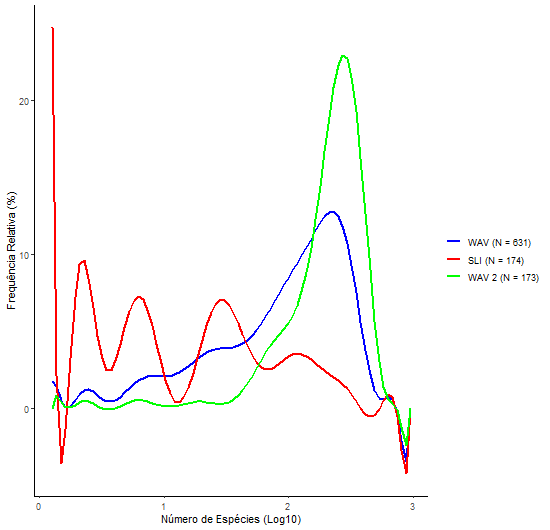
\includegraphics[height = 8cm]{Imagens/123.png}
\\{\scriptsize Figura 2: Distribuição de municípios em classes segundo o número de espécies (Log10), em cada banco de dados: WAV = Wikiaves, SLI = SpeciesLink, WAV2 = WAV com municípios redundantes em SLI. n = número de municípios. }
\end{figure}

\subsection{Registros por Espécie}

\begin{figure}[h!]
\centering
{\scriptsize Tabela 4: Estatísticas de tendência central e dispersão para o número de registros por espécie em cada banco de dados: WAV = Wikiaves, SLI = SpeciesLink, WAV2 = WAV com municípios redundantes em SLI. Valores de média (m) e desvio-padrão (dp) em Log10 foram retrotransformados (Retro). min-max = valores extremos, q1-q3 = quartis.}
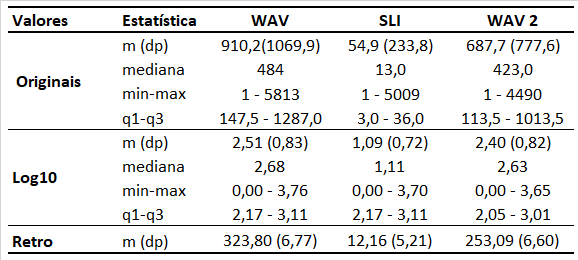
\includegraphics{Tabelas/4.png}
\end{figure}

\texto

\begin{figure}[h!]
\centering
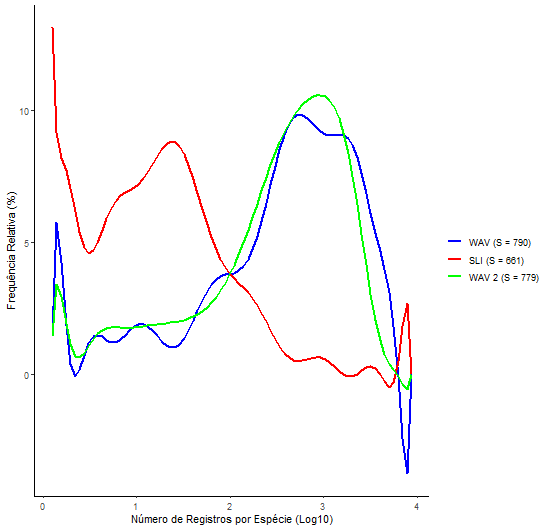
\includegraphics[height = 8cm]{Imagens/133.png}
\\{\scriptsize Figura 3: Distribuição de espécies em classes segundo o número de registros (Log10), em cada banco de dados: WAV = Wikiaves, SLI = SpeciesLink, WAV2 = WAV com municípios redundantes em SLI. S = número de espécies.}
\end{figure}

\newpage
